\chapter{A IMPORTÂNCIA DOS POLOS DE INOVAÇÃO}
\thispagestyle{empty}

\section{O modelo Universidade-Empresa-Governo}

Para \citeonline{saens2002ciencia} ciência pode ser definida por um método, uma instituição, uma tradição acumulativa de conhecimentos, um fator fundamental na manutenção e desenvolvimento da produção, e uma poderosa influência que deve refletir sua complexidade em diferentes aspectos na formação de crenças e atitudes relativas ao universo.

Compreende-se também que os avanços na ciência sempre estarão ligados a mudanças nas forças produtivas, e que por assim dizer estão diretamente ligados a inovação.

De acordo \citeonline{etzkowitz2003innovation}, a inovação pode ser linear, reversa, assistida ou interativa, ou um processo segue uma ordem natural em que a pesquisa científica básica, aplicada ou tecnológica será disponibilizado no mercado.

Em um modelo linear reverso as demandas da sociedade servem de ponto de iniciação de processo, enquanto no modelo linear assistido existe o desenvolvimento de mecanismos de apoio para a intermediação das capacidades de transferência de tecnologia, ou mesmo calculo de capital de risco. Existe ainda um modelo interativo que incorpora as características dos demais modelos, atendendo simultaneamente a diversas demandas e criando processos de apoio a inovação.

Nas últimas décadas os governos vêm criando incentivos a criação de ambientes de inovação, como incubadoras e projetos de pesquisa, que atuam dentro das universidades, sendo liderados muitas vezes pelos próprios projetos e com participação de empresas em diversos momentos, desde a criação desses projetos, ao oferecimento de mão de obra e/ou bolsas que suportem as pesquisas.

Essa missão que está voltada a trazer inovação para comunidade com bem competitivo e de eficiência veio através de um modelo desenvolvido a anos atrás.

Por volta do final dos anos 90, Henry Etzkovitz desenvolveu um modelo de inovação que visava explorar a relação UEG, este modelo veio a ser conhecido por tríplice hélice.

Neste modelo, as múltiplas relações consideradas recíprocas, eram dívidas em diferentes estágios de processo e disseminação de conhecimento de forma espiral, cada esfera representa uma instituição independente que trabalha em cooperação com as demais esferas, através de fluxos de conhecimento \cite{etzkowitz1998norms}.

\citeonline{etzkowitz2000dynamics} apresentaram uma visão da evolução dos SI, nas quais percebiam-se os conflitos potenciais nas relações de UEG. Portanto, essa nova visão trazia novas abordagens para essas variações nos arranjos institucionais dessas relações. A figura \ref{ueg_estatico} apresenta o modelo estático de relação UEG, onde o governo se envolve e passa a dirigir as relações entre as empresas e a Universidade.


\begin{figure}[ht]
  \centering
  \scalebox{0.7}{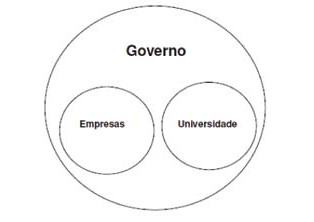
\includegraphics{figuras/ueg_estatico}}
  \caption{Modelo estático da relação UEG. Adaptado de \cite{etzkowitz2003innovation}.}
  \label{ueg_estatico}
\end{figure}

Uma segunda abordagem mostrada pela figura \ref{ueg_faire}, representa as relações completamente separadas entre as partes em suas esferas institucionais, assim estabelecendo relações por base de independência entre as partes. Essa abordagem também é conhecida por modelo “laissez-faire” de relação UEG.


\begin{figure}[ht]
  \centering
  \scalebox{0.7}{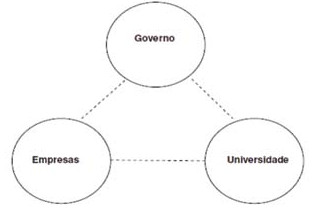
\includegraphics{figuras/ueg_faire}}
  \caption{Modelo \'laissez-faire\' da relação UEG. Adaptado de \cite{etzkowitz2003innovation}.}
  \label{ueg_faire}
\end{figure}

Na terceira abordagem, o conceito de geração de conhecimento é estruturado através da sobreposição das esferas institucionais, e portanto sobrepondo as ações das partes para estabelecer as condições de desenvolvimento de uma verdadeira relação produtiva. O objetivo é promover a inovação do ambiente na busca pelo conhecimento, pelo desenvolvimento econômico e por alianças estratégicas com empresas.

Neste memento o papel do governo deixa de ser controlar as outras esferas, e passa a ser estimular parcerias. Existe ainda um espaço para colaboração trilateral na formação de organizações híbridas, conforme visto na figura \ref{triplice_helice}.


\begin{figure}[ht]
  \centering
  \scalebox{0.7}{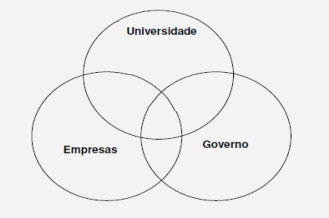
\includegraphics{figuras/triplice_helice}}
  \caption{Modelo da Tríplice Hélice na relação UEG. Adaptado de \cite{etzkowitz2003innovation}.}
  \label{triplice_helice}
\end{figure}

Neste último modelo também, universidade deixa de ser uma instituição centrada basicamente no ensino e combina seus recursos e potenciais na área de pesquisa com uma nova missão, desenvolver ideias de caráter econômico e social da sociedade, e assim estimula o surgimento de ambientes de inovação e dissemina uma cultura empreendedora.

Podem ser definidos como quatro os processos relacionados com as mudanças baseadas no conhecimento pela tríplice hélice \cite{etzkowitz2003innovation}:

\begin{itemize}
  \item{mudanças internas em cada esfera, tais como estratégias de cooperação ou alianças entre empresas concorrentes, ou a incorporação do desenvolvimento econômico e social como missão da universidade e o papel de articulador para o governo;}
  \item{reconhecimento da influência de cada esfera nas ações dos demais, seja essa influência por meio de legislações governamentais nas áreas de propriedade intelectual, ou transferência de tecnologia e inovação (Lei Bayh-Dole nos Estados Unidos e Lei da Inovação no Brasil);}
  \item{criação de novos relacionamentos entre as partes, sejam alianças estratégicas ou outras formas de cooperação que estimulem a criatividade e a inter-relação regional, e ainda a criação de ambientes de inovação;}
  \item{a ampliação e repercussão das ações da relação UEG junto à sociedade.}
\end{itemize}

Para \citeonline{etzkowitz1998norms} as universidades, e por assim dizer, formas de ensino, passaram por duas grandes revoluções desde a sua criação, época em que eram centradas na transmissão de conhecimentos dos professores para os alunos, sem um movimento de troca, apenas de repassamento de informações.

Na primeira revolução, que se deu no final do século 17, o conceito de pesquisa é agregado como missão das universidades, além das atividades de ensino. A princípio notou-se que muitos desafios ainda viriam antes de uma total incorporação das atividades de pesquisa no meio acadêmico.

Na segunda metade do século 20, mesmo com o ideal de pesquisa ainda não amadurecido, veio a segundo revolução que trouxe o conceito de Universidade empreendedora. Além da missão de ensino e pesquisa, neste memento mais um valor foi agregado como missão, o valor de formação de conhecimento voltado também ao desenvolvimento econômico e social.

Com este acréscimo a missão das universidades, houve uma proximidade entre essas e a sociedade, que começou a se sentir verdadeiramente inserida neste meio.

Alguns autores, como \citeonline{clark2003sustaining}, tratam a universidade empreendedora por Universidade inovadora, visto que a utilização de pesquisa e ciência permitem mudanças reais no mercado e portanto acarretam a inovação.

Assim, a concepção de universidade como simples “passadora” de conhecimento se modifica, se insere na sociedade, e passa a ser um dos principais papéis envolvidos na transformação de conhecimento gerado em valor econômico e social.

Entretanto, \citeonline{etzkowitz2003innovation} destaca que existem aspectos que prejudicam essa no época no ensino: na medida em que novos projetos surgem, conflitos de interesses também passar a surgir; esses conflitos de interesse podem ser decorrentes de interesses conflitantes, o não os ilegítima; assim a pesquisa e a comercialização dos resultados da pesquisa devem ser combinadas em um único modelo, visando evitar problemas.

Para \citeonline{clark2003sustaining} existem cinco fatores que endereçam questões críticas no processo de mudança nas universidades e portanto na relação UEG:

\begin{itemize}
  \item{a direção a seguir: no que respeito a estruturas gerenciais é preciso ter uma postura forte para que as mudanças sejam aceitas;}
  \item{o desenvolvimento expandido: é preciso estipular corretamente o desenvolvimento de novas estruturas frente as demandas da sociedade;}
  \item{as fontes de financiamento: diversificar as fontes de financiamento auxilia na ampliação dos recursos e portanto na estabilidade dos projetos;}
  \item{a estimulação das inovações: é preciso estimular os envolvidos nos processos de inovação para o processo seja bem aceito;}
  \item{a cultura empreendedora: é ideal criar uma cultura integrada, representada por uma visão compartilhada gerando uma perspectiva institucional.}
\end{itemize}

Assim, uma universidade empreendedora deve ser capaz de transformar pesquisa em resultados potenciais de comercialização, em ideias inovadoras tendo políticas de inovação como suporte de possibilidade de impacto regional.


\section{A relação UEG no Brasil}

No Brasil, durante os últimos 15 anos, tem existido um forte posicionamento em prol das atividades de PD\&I para inserção do meio acadêmico no dia a dia da sociedade frente as demandas da economia brasileira no mercado mundial e, desta forma, para estimular os SI, também entendidos como um conjunto de arranjos institucionais, cuja composição é dada pela relação UEG, levando à proposição de programas de incentivo à parceria \cite{vedovello2006capacidade, sbragia2006inovaccao}.

Entretanto, para \citeonline{toffler1990future}, nossos líderes políticos insistem no mito de o mercado, como sociedade industrial, esta destinado a perpetuar indefinidamente, e tristemente, muitos dos educadores, que por vezes são considerados agentes de mudança, dão continuidade a este pensamento. Assim, provavelmente, quando o futuro chegar junto a inovação essa ideia provará estar apenas obsoleta.

Essa preposição reforça que os SI sigam uma abordagem mais interativa, e menos linear, como o processo de empreendedorismo já antes citado por \citeonline{de2003introduccao}, que enfatiza um processo em que projetos podem ser apoiados por diferentes organizações, tanto privadas quanto governamentais.

Assim, podemos considerar que enquanto modelo de relação UEG, a tríplice hélice apresenta um arranjo organizacional bem evoluído por integrar a interação dessas três partes nos SI, e que serviu de ponto de partida para criação das Universidades Empreendedoras, como peças chaves para uma sociedade baseada no conhecimento \cite{etzkowitz2004evolution, etzkowitz2005innovating}.

No cenário internacional, diversos autores reconhecem o modelo da tríplice hélice como fator positivo no desenvolvimento regional e principal agente de inovação e transformação da ciência e tecnologia em crescimento econômico \cite{etzkowitz1998norms, etzkowitz2000dynamics, etzkowitz2007regional}.

Eles reconhecem ainda que esse crescimento da inovação esta diretamente ligado a capacidade de interação UEG prevista no modelo, bem como ao processo de aceitação da sociedade as mudanças na estrutura econômica.

Em suma, muitos estudos empíricos internacionais utilizaram seus esforços para estudar as relações e interações das partes frente a seu envolvimento, muitas vezes falhando em documentar sobre os aspectos da inovação em relação a sociedade.

\citeonline{tijssen2006universities} e \citeonline{welsh2008close} estudaram sobre como eram estabelecidas as relações entre as universidades e as empresas., \citeonline{campbell2005knowledge}, \citeonline{landry2006some}, \citeonline{mueller2006exploring} e \citeonline{welsh2008close} estudaram como se desenvolvia o recebimento e reinvestimento do suporte, ou fomento, recebido pelas universidades.

Por fim, sugeriram que a relação UEG pode afetar a performance e o desenvolvimento de ambas as partes de forma positiva, seja através da pesquisa, de patentes, ou desenvolvimento econômico \cite{landry2006some, mueller2006exploring, shane2004academic}.

\citeonline{sbragia2006inovaccao} avalia que no início, havia uma desconfiança mútua, fosse pela diferença de linguagem ou pelo choque de cultura, que resultava da falta de alinhamento entre as ideias e as imposições feitas pela pesquisa.

\citeonline{dagnino2003relaccao} levantaram um caso exemplar de relação UEG realizado pela Faculdade de Mecânica da Universidade Estadual de Campinas (FEM/Unicamp) com a então multinacional de autopeças Clark Equipaments. Inicialmente a proposta de interação veio através da realização de uma auditoria, posteriormente esta empresa se desenvolveu e se especializou de tal forma que veio a se desligar da filial se tornando Eaton Truck Corporation e vindo a firmar novos projetos tecnológicos com a participação da faculdade.

Através de um estudo que avaliou os dados do Diretório de pesquisa do CNPq no Censo 2002, \citeonline{rapini2007interaccao} destacou que existe a predominância de fluxos de conhecimento e serviços vindos de grupos de pesquisa para empresas, sendo esses serviços geralmente voltados a tarefas rotineiras de pouca complexidade. A autora destaca também que existe pouco uso do escopo de indicadores de CT\&I.

\citeonline{ipiranga2012tipo}, avaliaram a relação UEG através da Rede Nordeste Biotecnologia (Renorbio) e notaram que seu processo de cooperação era dotado de distinção de valores, linguagens, objetivos e cultura, o que tornava a interação entre as partes muito complexa, porém ativa para aqueles que estão diretamente envolvidos.

As autoras ainda destacam que um dos pontos que podem complexar a interação podem estar relacionados a falta de uma estrutura de gerenciamento, entretanto todos os resultados de pesquisa desenvolvidas estão patenteadas, demonstrando a viabilidade da inovação.

\citeonline{berni2015interaccao} relataram sobre a experiência vivida na Universidade Federal de Santa Maria (UFSM) pelo processo de incubadoras. De modo geral a experiência demonstrou ser positiva quanto a interação UEG, sendo mais voltado para as partes de universidade e empresa.

Para a empresa citou-se que houve auxílio ao desenvolvimento de novos produtos, enquanto para a universidade, houve o auxílio a formação de profissionais e possibilidades de direcionamento para aplicações práticas e interações com a comunidade.

\citeonline{etzkowitz2004evolution} e \citeonline{lundvall2010politicas} ressaltam que para alcançar o caminho da inovação é preciso cooperação de todas as partes, para que evoluam em um processo interativo e acumulativo que leva aos SI, sem cooperação não é possível compreender a distância entre o conhecimento e as diferentes  realidades da inovação.

Como \citeonline{ivanova2014rotational} ressaltam, é importante que o incentivo para o vinculo da relação UEG venha, sobretudo, da implementação de políticas governamentais, que tenham por objetivo garantir estrategias em diversas áreas que busquem a excelência e potencial contribuição para o crescimento econômico., assim como a melhoria de condição de vida no contexto regional e mesmo de nação \cite{lastres2005conhecimento}.

\section{A importância do PICG}

Para \citeonline{ristoff2011expansao} a Reforma Universitária garante que as universidades federais terão, enfim, a autonomia de gestão financeira prevista na constituição, mas nunca posta em prática; terão asseguradas a tão sonhada dotação global de recursos, a irredutibilidade nos repasses e a expansibilidade continuada.

Estarão, portanto, livres das amarras burocráticas e financeiras, que inibem a autogestão, repelem a inovação e forçam a privatização do espaço público. Ao defender a autonomia das universidades, nos termos do artigo 207 da Constituição, o governo também deixa claro o seu entendimento de que nestas instituições, embora não necessariamente nos Centros Universitários e Faculdades, as atividades de ensino, pesquisa e extensão são definidoras de sua natureza.

Em 2008, foram fundamentados os Institutos Federais (IF)\nomenclature{IF}{Institutos Federais} no país, para que fosse possível dar mais um passo no processo de expansão da Rede Federal de Educação, e também como parte dos objetivos de Plano de Desenvolvimento da Educação (PDE)\nomenclature{PDE}{Plano de Desenvolvimento da Educação} \cite{brasil2012ntextordmasculine, otranto2010criaccao}.

Um dos incentivos governamentais para conciliação de universidade, ou institutos, com empresas veio através da formalização da Empresa Brasileira de Pesquisa e Inovação Industrial (EMBRAPII)\nomenclature{EMBRAPII}{Empresa Brasileira de Pesquisa e Inovação Industrial} em 2013, para fomentar o processo de cooperação entre pequenas  e medias empresas nacionais e instituições tecnológicas ou privadas sem fins lucrativos.

Os primeiros projetos pilotos envolvem o Instituto de Pesquisa Tecnológico (IPT)\nomenclature{IPT}{Instituto de Pesquisa Tecnológico} na área de nanobiotecnologia, o Instituto Nacional de Tecnologia (INT)\nomenclature{INT}{Instituto Nacional de Tecnologia} em energia (gás/petróleo) e saúde e o Centro Integrado de Manufatura e Tecnologia (CIMATEC)\nomenclature{CIMATEC}{Centro Integrado de Manufatura e Tecnologia} do Serviço Nacional de Aprendizagem Industrial (SENAI)\nomenclature{SENAI}{Serviço Nacional de Aprendizagem Industrial} na área de automação manufatura.

Em março de 2015, a EMBRAPII selecionou cinco IF para atuarem em projetos de inovação industrial, para passarem pelo processo de seleção foi exigido das IF que participassem de um curso de capacitação de seus agentes de inovação, para que estivessem preparados para interagir com a relação UEG visando proporcionar eficiência  e agilidade no processo de transmissão de tecnologia para sociedade \cite{embrapiiff}.

Entre os polos selecionados destacasse o Polo de Inovação Campos dos Goytacazes pertencente ao Instituto Federal Fluminense (IFF)\nomenclature{IFF}{Instituto Federal Fluminense} em parceria com o Campus Rio Paraíba do Sul (UPEA)\nomenclature{UPEA}{Campus Rio Paraíba do Sul}, inicialmente Unidade de Pesquisa e Extensão Agroambiental.

Atualmente conhecido por PICG, o polo está localizado no município de Campos dos Goytacazes – RJ, no norte do estado do Rio de Janeiro, e foi reconhecido pelo Ministério da Educação em 13 de agosto de 2015 (PICG/IFFluminense – Portaria 819/2015). Desde sua inauguração a UPEA vem  realizando diversos trabalhos de fundamento ambiental para o atendimento das demandas regionais \cite{embrapiiff}.

Neste memento o PICG está sendo estruturado para desenvolver projeto de PD\&I e receberá um financiamento de R\$ 3 milhões para um plano de ação de 3 anos. Este plano de ação contará diretamente com a participação de empresas da região, visando transferir tecnologia para essas e, por fim, para a sociedade local \cite{embrapiiff}.
